
The goal of this paper is to analyze the correlation between the 10 year treasury yield and cryptocurrencies. The 10 year treasury rate is the yield one receives for investing in US government securities with a maturity of 10 years. It is a common proxy for the risk free rate. The risk free rate is a basic component of most pricing theories and thus a very relevant factor in the finance world. This paper will shed light on the influence of the risk free rate on the price of cryptocurrencies by analyzing price data over a period of 5 years. It will also be examined, wether the cryptocurrency market as a whole is affected.
\\

To answer the research question this paper looks at four different cryptocurrencies, namely Bitcoin, Etherium,  XRP (by Ripple) and Litecoin. Find an overview of the four currencies in Table 1 below.


\begin{table}[H]
\centering % Label your table accordingly
\begin{tabular}{>{\centering\arraybackslash}m{0.15\textwidth} >{\centering\arraybackslash}m{0.15\textwidth} >{\centering\arraybackslash}m{0.15\textwidth} >{\centering\arraybackslash}m{0.15\textwidth} >{\centering\arraybackslash}m{0.15\textwidth}}
\hline
Logo & Name & Symbol & Market Cap as of Nov 25, 2022 & Ranking as of Nov 25, 2022\\
\hline
\\
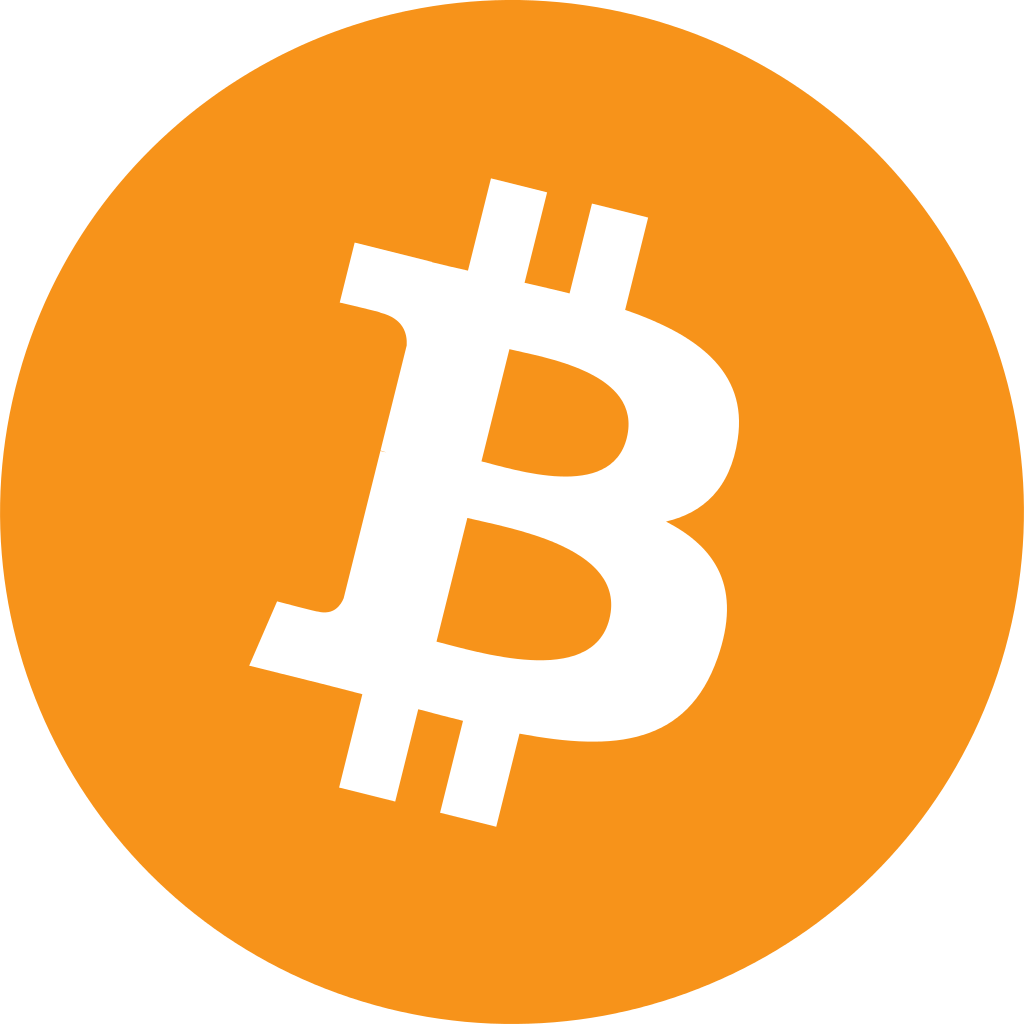
\includegraphics[width=0.1\textwidth]{images/Bitcoin.png} &  Bitcoin & BTC & \$ 318 bn & 1\\
\\
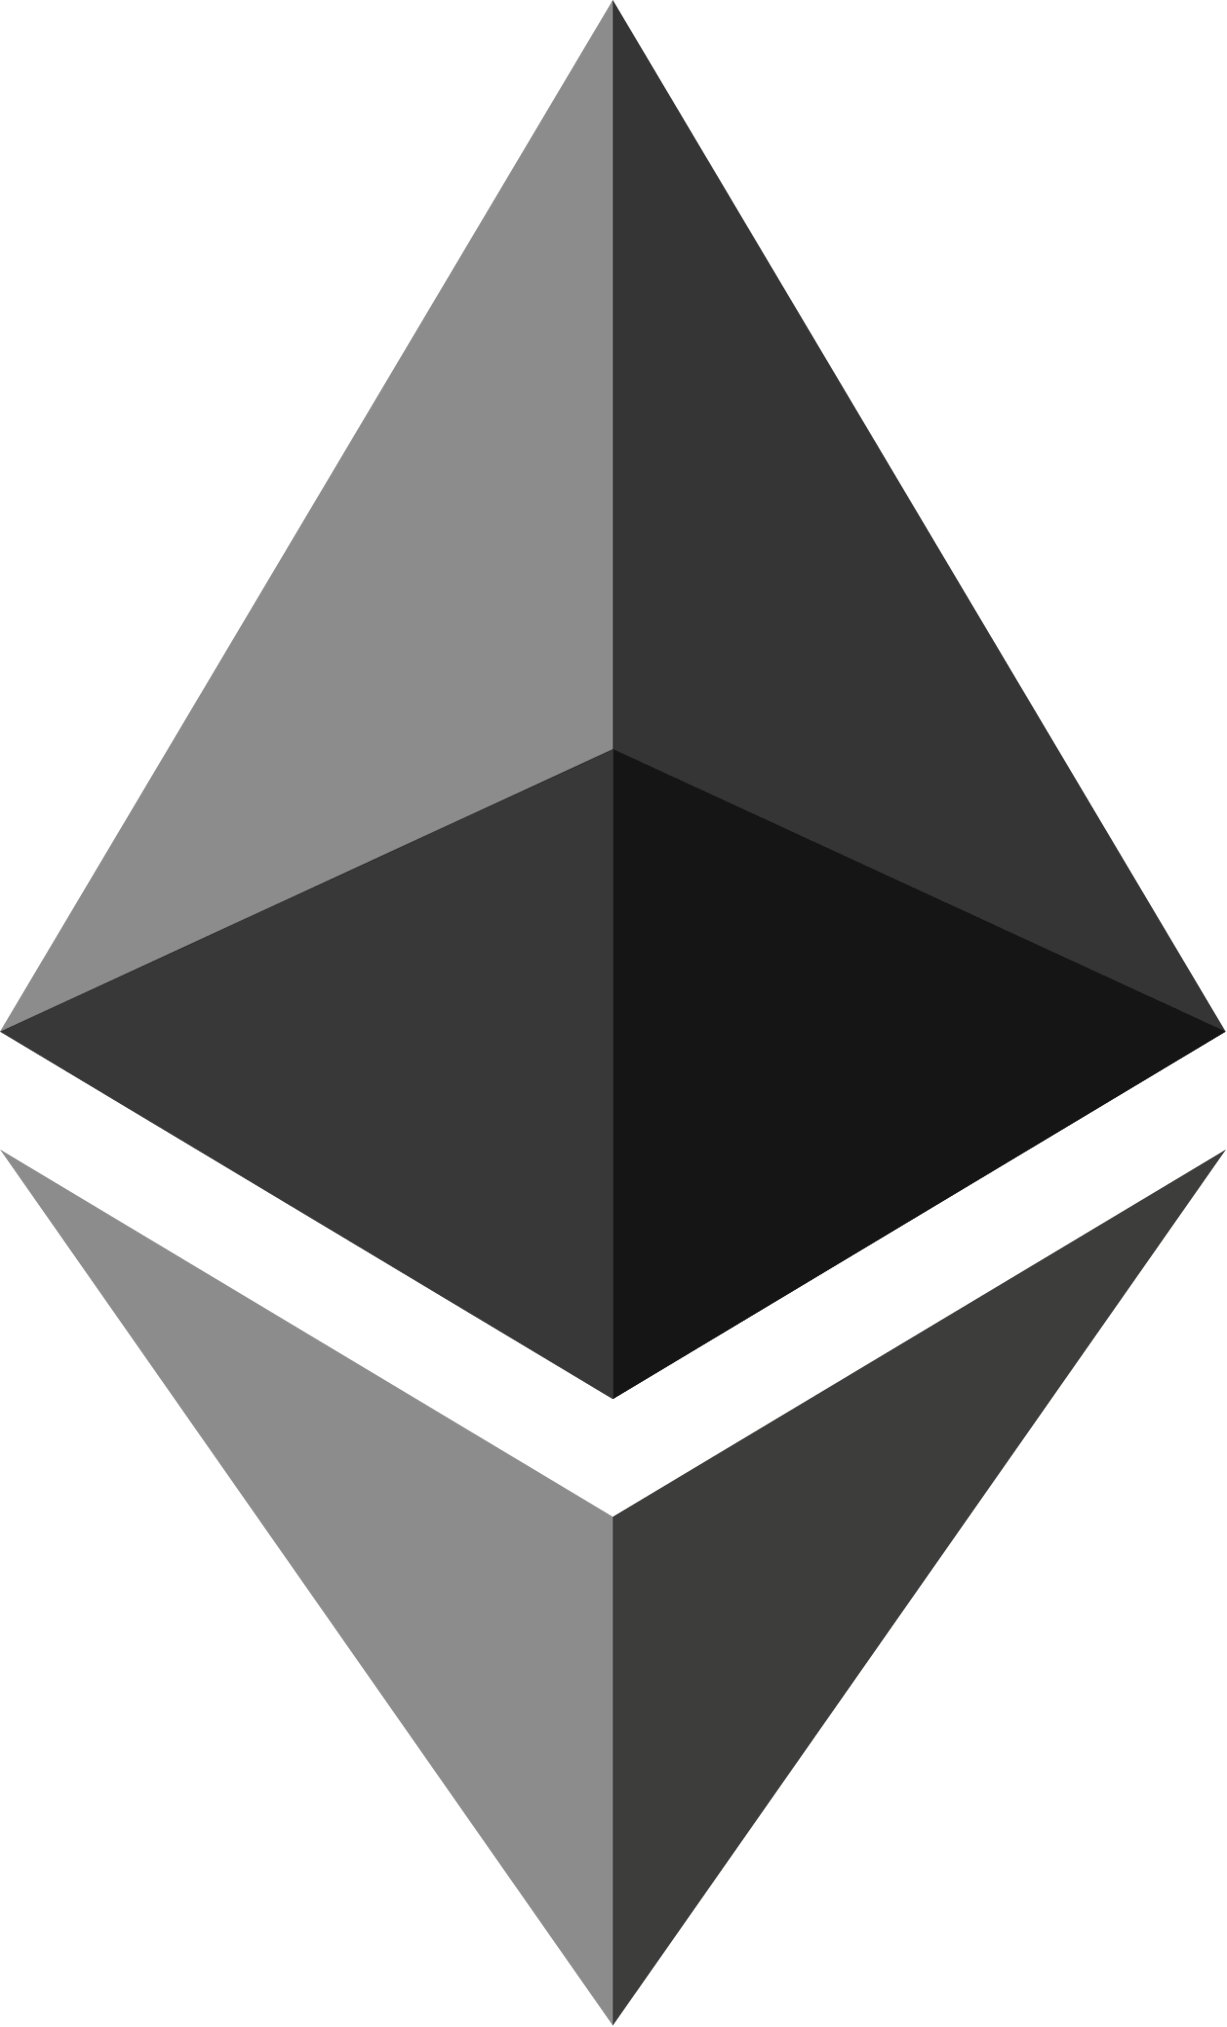
\includegraphics[width=0.05\textwidth]{images/ETH.png} & Ethereum & ETH & \$ 149 bn & 2\\
\\

\includegraphics[width=0.1\textwidth]{images/XRP.png} & XRP & XRP & \$ 20 bn & 7\\
\\

\includegraphics[width=0.1\textwidth]{images/LTC.png} & Litecoin & LTC & \$ 6 bn & 13\\
\\
\hline
\end{tabular}
\caption{\label{tab1} Cryptocurrencies. Quelle 2}
\end{table}


Besides these single cryptocurrencies, we also consider a cryptocurrency index. By looking at an index, we can replicate the cryptocurrency market as a whole and abstract from indiosyncratic risks of single currencies. The index that was considered is the CMC Crypto 200 Index by Solactive. The CMC Crypto 200 Index tracks the price movementes of the top 200 cryptocurrencies by market capitalization. It was launched at year end 2018 and is calculated and distributed by Solactive AG. The index is published in USD. The calculation of the index price is conducted on a daily basis (Quelle 1). As of November 2022, the four cryptocurrencies analyzed in this paper (Bitcoin, Etherium,  XRP and Litecoinwere) were within the 13 cryptocurrencies with the highest market capitalization and therefore also part of the CMC Crypto 200 (see Table 1).





\\

Quelle 1: https://www.solactive.com/wp-content/uploads/2019/04/Solactive-Index-Guideline-CMC200.pdf
Quelle 2: https://www.coingecko.com/

